%
% File coling2020.tex
%
% Contact: feiliu@cs.ucf.edu & liang.huang.sh@gmail.com
%% Based on the style files for COLING-2018, which were, in turn,
%% Based on the style files for COLING-2016, which were, in turn,
%% Based on the style files for COLING-2014, which were, in turn,
%% Based on the style files for ACL-2014, which were, in turn,
%% Based on the style files for ACL-2013, which were, in turn,
%% Based on the style files for ACL-2012, which were, in turn,
%% based on the style files for ACL-2011, which were, in turn, 
%% based on the style files for ACL-2010, which were, in turn, 
%% based on the style files for ACL-IJCNLP-2009, which were, in turn,
%% based on the style files for EACL-2009 and IJCNLP-2008...

%% Based on the style files for EACL 2006 by 
%%e.agirre@ehu.es or Sergi.Balari@uab.es
%% and that of ACL 08 by Joakim Nivre and Noah Smith

\documentclass[11pt]{article}
\usepackage{coling2020}
\usepackage{times}
\usepackage{url}
\usepackage{latexsym}
\usepackage{indentfirst}

\usepackage{times}
\usepackage{latexsym}
\usepackage{times}
\usepackage{soul}
\usepackage{url}
\usepackage{amsmath}
\usepackage{amsthm}
\usepackage{booktabs}
\usepackage{algorithm}
\usepackage{algorithmic}
\usepackage{amssymb}
\usepackage{longtable}
\usepackage{graphicx}
\usepackage{CJK}
\usepackage{multirow}
\usepackage{color}

%\setlength\titlebox{5cm}
\colingfinalcopy % Uncomment this line for the final submission

% You can expand the titlebox if you need extra space
% to show all the authors. Please do not make the titlebox
% smaller than 5cm (the original size); we will check this
% in the camera-ready version and ask you to change it back.


\title{2021年03月07日进度汇报}

\author{屈原斌 \\
  首都师范大学 \\
    {\tt ybqu@cnu.edu.cn}}

\date{}

\begin{document}
\begin{CJK}{UTF8}{gkai}

\maketitle
\CJKindent
%\begin{abstract}

%\end{abstract}

\section{今日进度}


\begin{itemize}
\item [1.] 完成英文BERT分类实验更新
\item [2.] 对比BERT取平均/CLS表示的离题指标
\item [3.] 中文BERT生成模型实验(中英文的都未跑完)
\item [4.] 好未来AI接口调用
\end{itemize}

\section{结论}
\begin{itemize}
  \item 英文BERT分类模型指标更新,见Table 1
  \item 离题实验:
  \begin{itemize}
    \item 方案一:基于题目排序方法,指标见Table2、3
    \item 方案一:基于相似度方法,指标见Table4、5
  \end{itemize}
  \item 结论:
  \begin{itemize}
    \item 加入测试集后离题指标下降
    \item 方案一中表示取平均方法离题指标优于CLS表示,方案二CLS表示更优
  \end{itemize}
\end{itemize}

% Table generated by Excel2LaTeX from sheet 'Sheet11'
\begin{table}[htbp]
  \centering
  \begin{tabular}{c|c|c|c|c}
    \hline
    & \textbf{Accuracy} & \textbf{Percision} & \textbf{Recall} & \textbf{F1-score} \\
    \hline
    \textbf{BERT} & 0.9198 & 0.9079 & 0.8954 & 0.8914 \\
    \hline
    \textbf{BERT(加入测试主题)} & 0.8805 & 0.8549 & 0.8414 & 0.8344 \\
    \hline
  \end{tabular}%
  \caption{Bert分类模型指标}
  \label{tab:addlabel}%
\end{table}%

% Table generated by Excel2LaTeX from sheet 'Sheet11'
\begin{table}[htbp]\small
  \centering
  \begin{tabular}{c|cc|ccc|ccc}
    \hline
    \multicolumn{3}{c}{\multirow{2}[0]{*}{\textcolor[rgb]{ 1,  0,  0}{}}} & \multicolumn{3}{c}{\textbf{离题}} & \multicolumn{3}{c}{\textbf{不离题}} \\
    \multicolumn{3}{c}{}  & \textbf{precision} & \textbf{recall} & \textbf{f1-score} & \textbf{precision} & \textbf{recall} & \textbf{f1-score} \\
    \hline
    \multirow{4}[0]{*}{\textbf{未加入测试集}} & \multirow{2}[0]{*}{\textbf{bert(取CLS)}} & \textbf{开发集} & 0.4676  & 0.6286  & 0.5346  & 0.5338  & 0.3737  & 0.4373  \\
    &       & \textbf{测试集} & 0.4665  & 0.6280  & 0.5352  & 0.5340  & 0.3725  & 0.4387  \\
    \cline{2-9}
    & \multirow{2}[0]{*}{\textbf{bert(取平均值)}} & \textbf{开发集} & 0.4666  & 0.5431  & 0.4995  & 0.5327  & 0.4562  & 0.4887  \\
    &       & \textbf{测试集} & 0.4647  & 0.5427  & 0.5005  & 0.5318  & 0.4539  & 0.4896  \\
    \hline
    \multirow{4}[0]{*}{\textbf{加入测试集}} & \multirow{2}[0]{*}{\textbf{bert(取CLS)}} & \textbf{开发集} & \multicolumn{1}{r}{0.4693 } & \multicolumn{1}{r}{0.1325 } & \multicolumn{1}{r}{0.2046 } & \multicolumn{1}{r}{0.5346 } & \multicolumn{1}{r}{0.8692 } & \multicolumn{1}{r}{0.6617 } \\
    &       & \textbf{测试集} & 0.4765  & 0.1367  & 0.2123  & 0.5354  & 0.8691  & 0.6626  \\
    \cline{2-9}
    & \multirow{2}[0]{*}{\textbf{bert(取平均值)}} & \textbf{开发集} & \multicolumn{1}{r}{0.4670 } & \multicolumn{1}{r}{0.1131 } & \multicolumn{1}{r}{0.1811 } & \multicolumn{1}{r}{0.5347 } & \multicolumn{1}{r}{0.8895 } & \multicolumn{1}{r}{0.6675 } \\
    &       & \textbf{测试集} & 0.4778  & 0.1161  & 0.1867  & 0.5353  & 0.8894  & 0.6683  \\
    \hline
    \end{tabular}%
  \caption{方案一指标更新(离题F1-score调阈值)}

  \label{tab:addlabel}%
\end{table}%

% Table generated by Excel2LaTeX from sheet 'Sheet12'
\begin{table}[htbp]\small
  \centering
    \begin{tabular}{c|cc|c|ccc|ccc}
      \hline
      \multicolumn{3}{c}{\multirow{2}[0]{*}{\textcolor[rgb]{ 1,  0,  0}{}}} & \multirow{2}[0]{*}{\textbf{Accurary}} & \multicolumn{3}{c}{\textbf{离题}} & \multicolumn{3}{c}{\textbf{不离题}} \\
      \multicolumn{3}{c}{}  &       & \textbf{precision} & \textbf{recall} & \textbf{f1-score} & \textbf{precision} & \textbf{recall} & \textbf{f1-score} \\
      \hline
      \multirow{4}[0]{*}{\textbf{未加入测试集}} & \multirow{2}[0]{*}{\textbf{bert(取CLS)}} & \textbf{开发集} & 0.5542  & 0.8030  & 0.1592  & 0.1885  & 0.5407  & 0.8742  & 0.6582  \\
      &       & \textbf{测试集} & 0.5361  & 0.7138  & 0.1690  & 0.1833  & 0.5428  & 0.8634  & 0.6469  \\
      \cline{2-10}
      & \multirow{2}[0]{*}{\textbf{bert(取平均值)}} & \textbf{开发集} & 0.5554  & 0.8024  & 0.1400  & 0.1723  & 0.5455  & 0.8970  & 0.6723  \\
      &       & \textbf{测试集} & 0.5331  & 0.7021  & 0.1446  & 0.1648  & 0.5387  & 0.8782  & 0.6545  \\
      \hline
      \multirow{4}[0]{*}{\textbf{加入测试集}} & \multirow{2}[0]{*}{\textbf{bert(取CLS)}} & \textbf{开发集} & 0.5627  & 0.7899  & 0.0996  & 0.1662  & 0.5509  & 0.9631  & 0.7004  \\
      &       & \textbf{测试集} & 0.5328  & 0.5998  & 0.0771  & 0.1270  & 0.5358  & 0.9315  & 0.6796  \\
      \cline{2-10}
      & \multirow{2}[0]{*}{\textbf{bert(取平均值)}} & \textbf{开发集} & 0.5530  & 0.8156  & 0.0643  & 0.1115  & 0.5446  & 0.9762  & 0.6988  \\
      &       & \textbf{测试集} & 0.5386  & 0.6359  & 0.0552  & 0.0977  & 0.5379  & 0.9614  & 0.6895  \\
      \hline
    \end{tabular}%
    \caption{方案一指标更新(Accuracy调阈值)}
  \label{tab:addlabel}%
\end{table}%

% Table generated by Excel2LaTeX from sheet 'Sheet11'
\begin{table}[htbp]\small
  \centering
    \begin{tabular}{c|cc|ccc|ccc}
      \hline
      \multicolumn{3}{c}{\multirow{2}[0]{*}{\textcolor[rgb]{ 1,  0,  0}{}}} & \multicolumn{3}{c}{\textbf{离题}} & \multicolumn{3}{c}{\textbf{不离题}} \\
      \multicolumn{3}{c}{}  & \textbf{precision} & \textbf{recall} & \textbf{f1-score} & \textbf{precision} & \textbf{recall} & \textbf{f1-score} \\
      \hline
      \multirow{4}[0]{*}{\textbf{未加入测试集}} & \multirow{2}[0]{*}{\textbf{bert(取CLS)}} & \textbf{开发集} & 0.4722  & 0.9803  & 0.6367  & 0.1462  & 0.0400  & 0.0628  \\
      &       & \textbf{测试集} & 0.4671  & 0.9677  & 0.6291  & 0.1089  & 0.0351  & 0.0530  \\
      \cline{2-9}
      & \multirow{2}[0]{*}{\textbf{bert(取平均值)}} & \textbf{开发集} & 0.4906  & 0.9408  & 0.6388  & 0.1440  & 0.1137  & 0.1271  \\
      &       & \textbf{测试集} & 0.4731  & 0.9266  & 0.6200  & 0.1147  & 0.0897  & 0.1006  \\
      \hline
      \multirow{4}[0]{*}{\textbf{加入测试集}} & \multirow{2}[0]{*}{\textbf{bert(取CLS)}} & \textbf{开发集} & 0.4663  & 1.0000  & 0.6352  & 0.0000  & 0.0000  & 0.0000  \\
      &       & \textbf{测试集} & 0.4663  & 1.0000  & 0.6359  & 0.0000  & 0.0000  & 0.0000  \\
      \cline{2-9}
      & \multirow{2}[0]{*}{\textbf{bert(取平均值)}} & \textbf{开发集} & 0.4663  & 1.0000  & 0.6352  & 0.0000  & 0.0000  & 0.0000  \\
      &       & \textbf{测试集} & 0.4663  & 1.0000  & 0.6359  & 0.0000  & 0.0000  & 0.0000  \\
      \hline
    \end{tabular}%
    \caption{方案二指标更新(离题F1-score调阈值)}
  \label{tab:addlabel}%
\end{table}%

% Table generated by Excel2LaTeX from sheet 'Sheet12'
\begin{table}[htbp]\small
  \centering
  \caption{Add caption}
  \begin{tabular}{c|cc|c|ccc|ccc}
    \hline
    \multicolumn{3}{c}{\multirow{2}[0]{*}{\textcolor[rgb]{ 1,  0,  0}{}}} & \multirow{2}[0]{*}{\textbf{Accurary}} & \multicolumn{3}{c}{\textbf{离题}} & \multicolumn{3}{c}{\textbf{不离题}} \\
    \multicolumn{3}{c}{}  &       & \textbf{precision} & \textbf{recall} & \textbf{f1-score} & \textbf{precision} & \textbf{recall} & \textbf{f1-score} \\
    \hline
    \multirow{4}[0]{*}{\textbf{未加入测试集}} & \multirow{2}[0]{*}{\textbf{bert(取CLS)}} & \textbf{开发集} & 0.5747  & 0.4841  & 0.4578  & 0.4233  & 0.5719  & 0.7348  & 0.6268  \\
    &       & \textbf{测试集} & 0.5241  & 0.5926  & 0.2641  & 0.2977  & 0.5508  & 0.7786  & 0.6283  \\
    \cline{2-10}
    & \multirow{2}[0]{*}{\textbf{bert(取平均值)}} & \textbf{开发集} & 0.5855  & 0.4970  & 0.3595  & 0.3861  & 0.5921  & 0.7737  & 0.6551  \\
    &       & \textbf{测试集} & 0.5452  & 0.4279  & 0.3398  & 0.3452  & 0.5668  & 0.7275  & 0.6149  \\
    \hline
    \multirow{4}[0]{*}{\textbf{加入测试集}} & \multirow{2}[0]{*}{\textbf{bert(取CLS)}} & \textbf{开发集} & 0.5723  & 0.8515  & 0.1219  & 0.1890  & 0.5565  & 0.9563  & 0.7033  \\
    &       & \textbf{测试集} & 0.5407  & 0.6537  & 0.0880  & 0.1429  & 0.5405  & 0.9375  & 0.6847  \\
    \cline{2-10}
    & \multirow{2}[0]{*}{\textbf{bert(取平均值)}} & \textbf{开发集} & 0.5735  & 0.7761  & 0.1309  & 0.2091  & 0.5575  & 0.9524  & 0.7032  \\
    &       & \textbf{测试集} & 0.5443  & 0.6659  & 0.0910  & 0.1508  & 0.5425  & 0.9412  & 0.6876  \\
    \hline
    \end{tabular}%
    \caption{方案二指标更新(Accuracy调阈值)}
  \label{tab:addlabel}%
\end{table}%


% Table generated by Excel2LaTeX from sheet '中文数据集'
% \begin{figure*}[htbp]\small
%   \centering
%   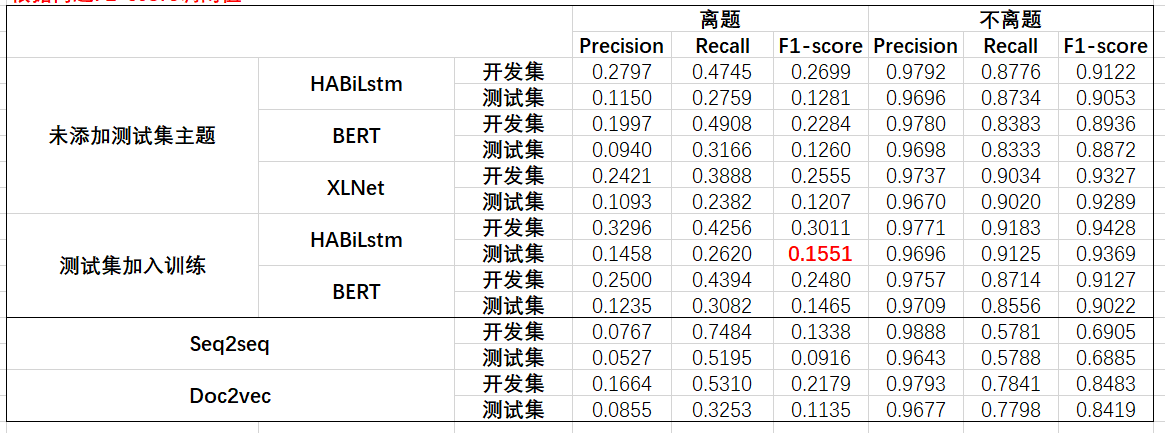
\includegraphics[width=1.0\linewidth]{zb.png}
%   \caption{生成样例2}
%   \label{framework}
% \end{figure*}

%\bibliography{reference}
%\bibliographystyle{coling}
%\bibliography{coling2020}

\end{CJK}
\end{document}


% include your own bib file like this:


%\begin{thebibliography}{}

%\bibitem[\protect\citename{Aho and Ullman}1972]{Aho:72}
%Alfred~V. Aho and Jeffrey~D. Ullman.
%\newblock 1972.
%\newblock {\em The Theory of Parsing, Translation and Compiling}, volume~1.
%\newblock Prentice-{Hall}, Englewood Cliffs, NJ.

%\bibitem[\protect\citename{{American Psychological Association}}1983]{APA:83}
%{American Psychological Association}.
%\newblock 1983.
%\newblock {\em Publications Manual}.
%\newblock American Psychological Association, Washington, DC.

%\bibitem[\protect\citename{{Association for Computing Machinery}}1983]{ACM:83}
%{Association for Computing Machinery}.
%\newblock 1983.
%\newblock {\em Computing Reviews}, 24(11):503--512.

%\bibitem[\protect\citename{Chandra \bgroup et al.\egroup }1981]{Chandra:81}
%Ashok~K. Chandra, Dexter~C. Kozen, and Larry~J. Stockmeyer.
%\newblock 1981.
%\newblock Alternation.
%\newblock {\em Journal of the Association for Computing Machinery},
%  28(1):114--133.

%\bibitem[\protect\citename{Gusfield}1997]{Gusfield:97}
%Dan Gusfield.
%\newblock 1997.
%\newblock {\em Algorithms on Strings, Trees and Sequences}.
%\newblock Cambridge University Press, Cambridge, UK.

%\bibitem[\protect\citename{Rasooli and Tetreault}2015]{rasooli-tetrault-2015}
%Mohammad~Sadegh Rasooli and Joel~R. Tetreault. 2015.
%\newblock {Yara parser: {A} fast and accurate dependency parser}.
%\newblock \emph{Computing Research Repository}, arXiv:1503.06733.
%\newblock Version 2.

%\bibitem[\protect\citename{Borschinger and Johnson}2011]{borsch2011}
%Benjamin Borschinger and Mark Johnson. 2011.
%\newblock A particle filter algorithm for {B}ayesian wordsegmentation.
%\newblock In \emph{Proceedings of the Australasian Language Technology Association %Workshop 2011}, pages 10--18, Canberra, Australia.

%\end{thebibliography}

